\documentclass[10pt]{beamer}
\usetheme{default}
\setbeamertemplate{navigation symbols}{}
\setbeamertemplate{footline}
{
  \leavevmode%
  \hbox{%
  \begin{beamercolorbox}[wd=.40\paperwidth,ht=2.5ex,dp=1ex,center]{author in head/foot}%
    \usebeamerfont{author in head/foot}\insertshortauthor
  \end{beamercolorbox}%
  \begin{beamercolorbox}[wd=.50\paperwidth,ht=2.5ex,dp=1ex,center]{title in head/foot}%
    \usebeamerfont{title in head/foot}\insertshorttitle
  \end{beamercolorbox}%
  \begin{beamercolorbox}[wd=.10\paperwidth,ht=2.5ex,dp=1ex,center]{date in head/foot}%
    \insertframenumber{} /\inserttotalframenumber\hspace*{1ex}
  \end{beamercolorbox}}%
  \vskip0pt%
}
\makeatletter

\usepackage[T1]{fontenc}
%\usepackage[utf8]{inputenc}
%\usepacage[italian]{babel}
\usepackage{amsmath} % allows to use \text in arrays
\usepackage{afterpage} % Execute command after the next page break
\usepackage{syntonly}
%\syntaxonly
\usepackage{changepage}
\usepackage{comment}

%Tables and figures
\usepackage{tabularx} % introduces column type X
\usepackage{tabularray}
\usepackage{array}
\usepackage{rotating} % per ruotare tabelle grandi
\usepackage{longtable}
\usepackage{siunitx} % gestisce in modo molto potente e flessibile anche la resa tipografica dei numeri nelle tabelle, definendo un nuovo tipo di colonna S specifica per dati numerici
\sisetup{output-decimal-marker={.},input-symbols = ()} % "(" and ")" are ordinary inputs
\setbeamertemplate{caption}[numbered]
\setbeamerfont{framesubtitle}{size=\large}
\usepackage[compatibility=false]{caption}
\captionsetup{tableposition=top,figureposition=bottom,font=scriptsize}
\usepackage{subcaption}
\captionsetup[sub]{font=scriptsize,labelfont={bf,sf}}
\usepackage{booktabs} % per tabelle
\usepackage{graphicx} % per figure
\usepackage{pgfplots}
\pgfplotsset{width=\textwidth,compat=1.11}
\usepackage{adjustbox}
\usepackage{tikz}
\usetikzlibrary{calc}
\graphicspath{{../paper/}{../figures/}{../}}
\usepackage{threeparttable}

%New command for captions below the table (in addition to those above)
\newcommand\fnote[1]{\captionsetup{format=plain,font=footnotesize,justification=justified}\caption*{#1}}
\newcommand{\B}[1]{{\color{blue} #1}}
\newcommand{\G}[1]{{\color{gray} #1}}
\hypersetup{colorlinks=true, breaklinks=false, linkcolor=gray, menucolor=gray, urlcolor=blue, citecolor=gray}

%Symbols
\usepackage{pifont}% http://ctan.org/pkg/pifont
\newcommand{\cmark}{\ding{51}}%
\newcommand{\xmark}{\ding{55}}%

%% Referencing
\usepackage{hyperref}
%\usepackage{breqn}
%\usepackage{amsmath}

%% Citations
%\usepackage[authoryear]{natbib}
%\usepackage{hyperref}
%\citestyle{apacite}
%\def\bibfont{\small}

%Biblio
\usepackage[style=authoryear-comp,backend=bibtex,uniquename=init,firstinits,maxcitenames=2,natbib=true,url=false,doi=false,eprint=false]{biblatex}
\bibliography{bibliography}

\title[Institutions and innovation]{Institutions and Innovation: \\ Evidence from the Italian Unification}

\author[Domini \& Machielsen]{Giacomo Domini\inst{} 
    \and Bas Machielsen\inst{}}

\institute{
    \inst{} Utrecht University School of Economics}
    
\date[May 2024]{Applied Economics seminar, 23 May 2024}

\begin{document}

\begin{frame}
  \titlepage
\end{frame}

\begin{frame}
    \frametitle{Introduction}
    
    Innovation seen at the basis of economic growth (Schumpeter, 1942; Solow, 1957) \\  \bigskip
    
    Innovation is a \textit{proximate} cause of economic growth; it is itself determined by \textit{fundamental} causes, most importantly institutions (Acemoglu  et al., 2005; North and Thomas, 1973; North, 1990) \\    \bigskip
    
    \pause
    
    19th-century Europe: many episodes of institutional change, at a time in which the First Industrial Revolution spread and the Second  started \\    \bigskip

    We focus on an episode from Italy's unification process (1850-60s), namely the annexation of Lombardy to Piedmont from Austria:
    
    \begin{itemize}
        \item Significant shift towards liberal institutions
        \item Quasi-random assignment, based on military circumstances
    \end{itemize}

    \bigskip
    
    Not only of historical relevance, at an age characterised by serious challenges to the liberal-democratic global order 
    
\end{frame}

\begin{frame}
    \frametitle{Relevant literature}
    
    Institutions and economic growth (Acemoglu et al., 2001; Rodrik et al., 2004) \\  \bigskip

    Institutions and innovation (Donges et al., 2022; Acemoglu \& Johnson, 2023)
    \begin{itemize}
        \item National innovation systems (Freeman, 1987; Lundvall, 1992; Nelson, 1993)
    \end{itemize}
    
    \bigskip

    Democracy and innovation (Aghion et al., 2007; Acemoglu et al., 2019)
    \begin{itemize}
        \item The "Popper" hypothesis (Gao et al., 2017; Wang et al., 2021) 
        \item Homophily preference (Mokyr, 2024)
    \end{itemize}
    
    \bigskip

    Innovation in post-Unification Italy (Barbiellini Amidei et al., 2013; Toninelli and Vasta 2014; Nuvolari and Vasta, 2015; 2017; Nuvolari et al., 2018; Domini, 2023)
    
\end{frame}

\begin{frame}
    \frametitle{Historical context}
    
    \begin{figure}
        \centering
        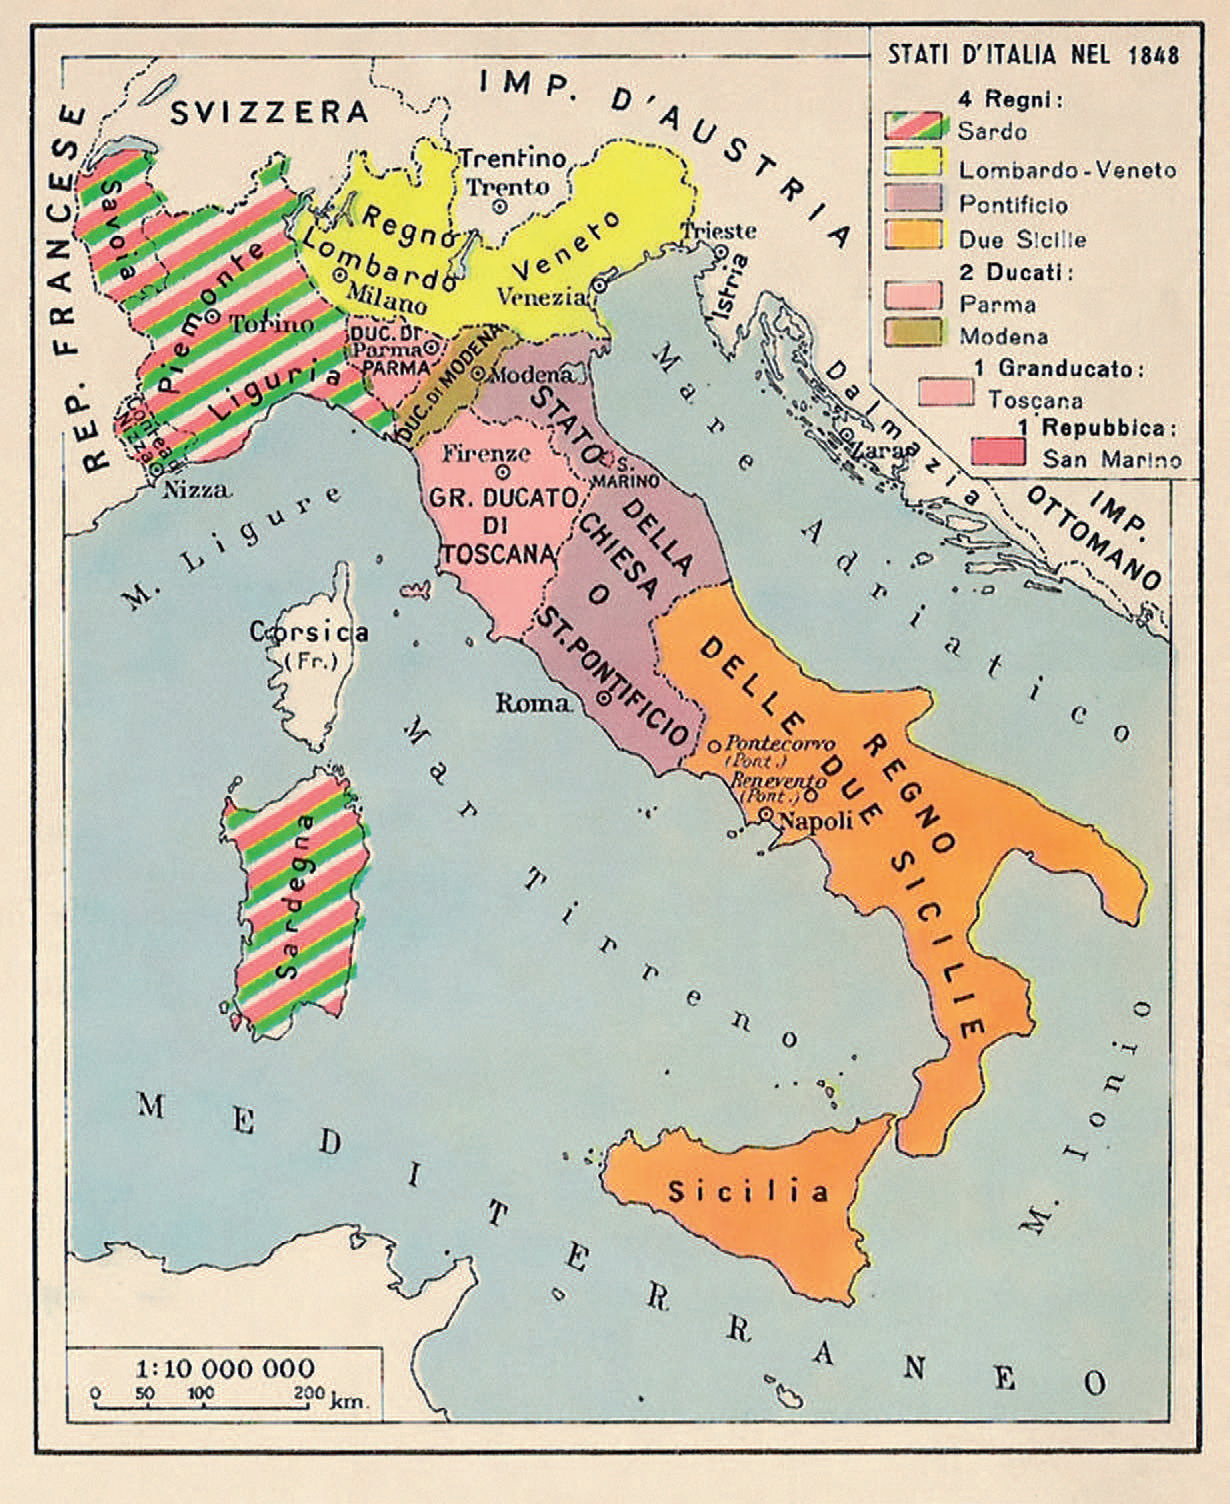
\includegraphics[width=0.5\linewidth]{maps/stati_preunitari.png}
        \caption{Italy in 1848}
        \label{fig:map_italy_1848}
    \end{figure}
    
\end{frame}

\begin{frame}
    \frametitle{Historical context}
    
    \begin{figure}
        \centering
        \includegraphics[width=0.75\linewidth]{maps/austrian_empire_1855.jpg}
        \caption{The Austrian empire in 1855}
        \label{fig:map_austria_1855}
    \end{figure}
    
\end{frame}

\begin{frame}
    \frametitle{Historical context}
    
    \begin{figure}
        \centering
        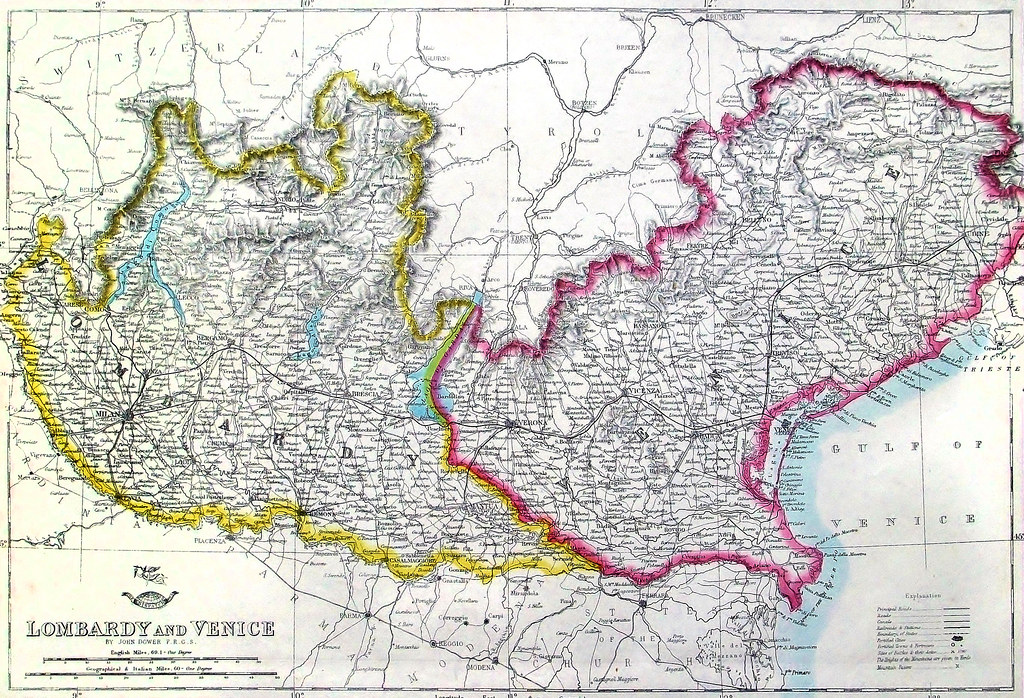
\includegraphics[width=0.75\linewidth]{maps/lombardy_venice}
        \caption{The Lombardo-Venetian kingdom}
        \label{fig:map_lombardy_venice}
    \end{figure}
    
\end{frame}

\begin{frame}
    \frametitle{Historical context}
    
    \begin{itemize}
        \item Italy last united under Justinian (mid-6th c.)
        \item Fragmented but flourishing until 15th c.
        \item Long political and economic decline in early modern period $\rightarrow$ Ruled by France, Spain, Austria
        \item In the wake of the French Revolution, growing sentiment in favour of national independence and unification (\textit{Risorgimento})
        \pause
        \item 1848-1849: uprisings and first war of independence (lost)
        \item \textbf{1859: second war of independence $\rightarrow$ Lombardy joins Piedmont}
        \item 1860: Garibaldi conquers the South
        \item 1859-1860: plebiscites across the peninsula to join Piedmont
        \item 1861: Vittorio Emanuele II proclaimed King of Italy
        \item 1866: third war of independence: Veneto joins
        \item 1870: Rome is captured and becomes capital
        \item Post-WWI: Trento and Trieste join
    \end{itemize}
    
\end{frame}

\begin{frame}
    \frametitle{Historical context: the second war of independence}
    
    Piedmont (formally the Kingdom of Sardinia) led the unification:
    \begin{itemize}
        \item Stable monarchy of the House of Savoy
        \item The only Italian state not to repeal the constitution in 1848-9
        \item Liberalism, free trade, compulsory universal schooling (since 1859)
    \end{itemize}

    \pause
    
    \bigskip

    Plombières agreement (1858) and Franco-Piedmontese military alliance (1859): France would help freeing the Lombardo-Venetian kingdom and get Savoy and Nice as reward

    \bigskip
    War fought over 2.5 months (25/4-12/7/1859)
    \begin{itemize}
        \item Austria first enters Piedmont, then retreats as French and Piedmontese advance
        \item After victory in Solferino (south of the Garda Lake), Napoleon III signs armistice with Austria: Lombardy (but Mantua) ceded to France, then to Piedmont
        \item Piedmont's PM Cavour resigns over unsatisfactory outcome
    \end{itemize}
    
\end{frame}

\begin{frame}
    \frametitle{The border}
    %La frontiera, partendo dal limite meridionale del Tirolo, sul lago di Garda, seguirà il \textbf{mezzo del lago} fino all’altezza di Bardolino e di Manerba; ove essa raggiungerà in linea retta il punto di intersecazione della zona di difesa della piazza di \textbf{Peschiera} con il lago di Garda. Questa zona sarà determinata da una \textbf{circonferenza il cui raggio calcolato a partire dal centro della piazza, è fissato a 3,500 metri}, più la distanza del detto centro alla spianata del forte il più avanzato. Dal punto d’intersecazione della circonferenza così disegnata col \textbf{Mincio}, la frontiera seguirà il \textbf{Thalweg della riviera fino alle Grazie}, si estenderà dalle Grazie in \textbf{linea diretta, fino a Scarzarolo}, seguirà il \textbf{Thalweg del Po fino a Luzzara}, punto a partire dal quale non è nulla cambiato ai limiti attuali, tali quali esistevano prima della guerra. (From art.  4 of the Treaty of Zurich, 10 November 1859)

    \begin{figure}
        \centering
        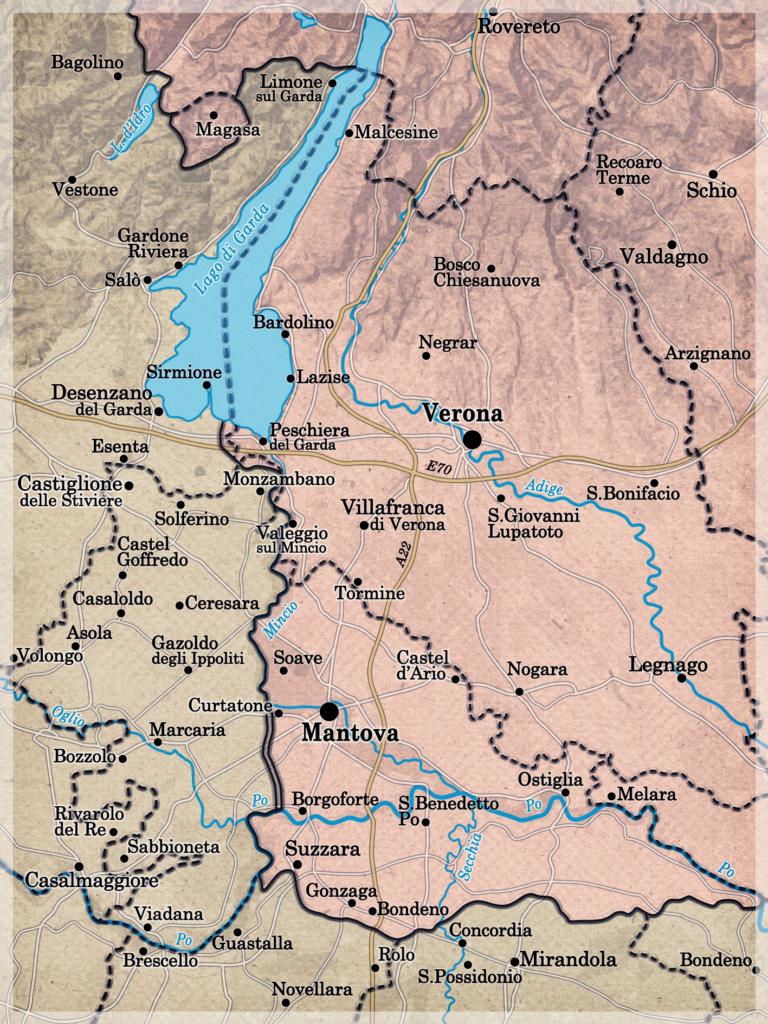
\includegraphics[width=0.5\linewidth]{maps/border.png}
        \caption{The border after the war in 1859}
        \label{fig:border}
    \end{figure}

\end{frame}

\begin{frame}
    \frametitle{The treatment: a comparison of constitutions}
    
    Piedmont's \textit{Statuto Albertino} (1848-1947):
    \begin{itemize}
        \item ``Representative monarchy'' with appointed upper chamber and elective lower chamber 
        \item King formally owns executive power; in practice, strong PMs (notably Cavour)
        \item Equality, individual liberty, free press, inviolability of private property
    \end{itemize}

    \pause
    \bigskip
    
    Meanwhile, in Austria: Pillersdorfs Constitution (1848), March Constitution (1848-1851), none (1852-1860), October Diploma (1860), \textbf{February Patent (1861-1865)}, December Constitution (1867-1918)

    \begin{itemize}
        \item One chamber appointed, one indirectly elected (by provincial diets) 
        \item ``The right to enact, amend or repeal laws shall only be exercised with the participation of the Diet or the Imperial Council''
        \item Liberal newspaper \textit{Wanderer} (1864): ``[S]ince 1861 ... a constitution without freedom of association, without jury courts, without freedom of press, without equality of confessional rights, lacking a reform of justice and administration''
    \end{itemize}

\end{frame}

\begin{frame}
    \frametitle{The treatment: other dimensions}
    
    The transfer of Lombardy from Austria to Piedmont/Italy represented a shock also along other dimensions relevant to innovation, in particular:

    \begin{itemize}
        \item Innovation institutions, e.g. patent system

        \begin{itemize}
            \item Both were French-inspired registration systems
            \item Italian \textit{privative industriali} some 10-15\% cheaper than Austrian \textit{Privilegien}  
        \end{itemize}

        \item Market potential (Missiaia, 2016)
        \item Cultural affinity of new state (on homophily and innovation, see Ertug et al., 2021)
    \end{itemize}
    
\end{frame}

\begin{frame}[label = patent_fees]
    \frametitle{Patent fees}

\begin{table}[!h]
\caption{\label{tab:pat_fees} Patent fees in Austria and Italy (post-1859)}
\centering
\fontsize{8}{8}\selectfont

    \begin{tabular}{cccccccc}
        \hline
        Years & \multicolumn{2}{c}{Yearly fee (GBP)} &   & \multicolumn{2}{c}{Cumulative fee (GBP)} &   & Rel. diff. (\%) \\
        \cline{2-3}\cline{5-6}  & Austria & Italy &   & Austria & Italy &   &  \\
        \hline
        1 & 2 & 1.67 &   & 2 & 1.67 &   & -16.67 \\
        2 & 2 & 1.67 &   & 4 & 3.33 &   & -16.67 \\
        3 & 2 & 1.67 &   & 6 & 5.00 &   & -16.67 \\
        4 & 2 & 2.50 &   & 8 & 7.50 &   & -6.25 \\
        5 & 2 & 2.50 &   & 10 & 10.00 &   & 0.00 \\
        6 & 3 & 2.50 &   & 13 & 12.50 &   & -3.85 \\
        7 & 3.5 & 3.33 &   & 16.5 & 15.83 &   & -4.04 \\
        8 & 4 & 3.33 &   & 20.5 & 19.17 &   & -6.50 \\
        9 & 4.5 & 3.33 &   & 25 & 22.50 &   & -10.00 \\
        10 & 5 & 4.17 &   & 30 & 26.67 &   & -11.11 \\
        11 & 6 & 4.17 &   & 36 & 30.83 &   & -14.35 \\
        12 & 7 & 4.17 &   & 43 & 35.00 &   & -18.60 \\
        13 & 8 & 5.00 &   & 51 & 40.00 &   & -21.57 \\
        14 & 9 & 5.00 &   & 60 & 45.00 &   & -25.00 \\
        15 & 10 & 5.00 &   & 70 & 50.00 &   & -28.57 \\
        \hline
    \end{tabular}%
        
    Source: own elaboration based on Tolhausen (1868).

\smallskip
\raggedright Average difference = -13.3\%, based on distribution of patents for 1902 \hyperlink{duration}{\beamergotobutton{Graphs}}  \\
Note: slightly downward biased since extension fees (as well as completion and reduction) are not taken into account.
    
\end{table}
    
\end{frame}



    
\begin{frame}
    \frametitle{Data}
    
    We proxy innovation by:

    \begin{itemize}
        \item \textbf{Patents}: standard gauge, especially in historical settings (Streb, 2023), but: (1) invention, not innovation; (2) not all inventions are patented, with propensity to patent widely varying (Griliches 1990; Nagaoka et al. 2010)
        
        \begin{itemize}
            \item Piedmont/Italy and Austria
        \end{itemize}

        \pause
        
        \item Exhibits at \textbf{universal exhibitions} can capture innovation with and without patents (Moser, 2005; 2011; 2012); but may suffer from opposite drawbacks with respect to patents and rather be informative about production structure (Domini, 2019; 2022; 2023)
         
        \begin{itemize}
            \item Catalogues from Paris 1855, 1867, 1878, 1889, and 1900, plus Turin 1911
            \item More granular than patents! Italy, 1867: 431 patents, 3841 exhibits 
        \end{itemize}

    \end{itemize}

    \bigskip
    In both cases, data collection still partly ongoing
    
\end{frame}

\begin{frame}
    \frametitle{Empirical strategy}
    
    Exogenous assignment of the new border $\rightarrow$ (cross-sectional) regression discontinuity (RD) design:    

    \begin{equation*}
        Y_{i} = \alpha + \beta D_i + \gamma Dist_i + \epsilon_i 
    \end{equation*}

    \bigskip
    
    Difference in differences (DD) also possible:

    \begin{equation*}
        Y_{it} = \alpha_i + \beta_1 \text{Post}_t + \beta_2 D_i \cdot \text{Post}_t + \epsilon_{it}
    \end{equation*}

    \bigskip

    The dependent variable is:

    \begin{itemize}
    
        \item Sum of Austrian and Italian patents
        \begin{itemize}
            \item To account for ``patenting diversion''
        \end{itemize}

        \item Number of exhibits
        \begin{itemize}
            \item Not the preferred measure (different sizes of exhibitions a/o location contingents)
            \item Alternative: mean or top product complexity (Hidalgo and Hausmann, 2009; Domini, 2022) 
        \end{itemize}
    
    \end{itemize}
    
    \bigskip

\end{frame}

\begin{frame}
    \frametitle{Lombardy and Veneto before the war}

\begin{table}[!h]
\caption{The Lombardo-Venetian provinces, 1857, \%}
\centering
\fontsize{8}{8}\selectfont

    \begin{tabular}{l r r r r r r}  
        \toprule
        Province & Pop. & Pop./Ha & Urb. & Agr. & Ind. & Serv.    \\ 
        \midrule
        Bergamo & 0.39 & 0.98 & 0.07 & 0.68 & 0.17 & 0.15 \\
        \textit{Brescia} & 0.36 & 1.16 & 0.12 & 0.54 & 0.23 & 0.23 \\
        Como & 0.44 & 1.60 & 0.04 & 0.71 & 0.16 & 0.13 \\
        Cremona & 0.21 & 1.57 & 0.14 & 0.59 & 0.22 & 0.19 \\
        Lodi e Crema & 0.22 & 1.90 & 0.08 & 0.6 & 0.21 & 0.2 \\
        \textit{Mantova} & 0.26 & 1.13 & 0.11 & 0.65 & 0.19 & 0.16 \\
        Milano & 0.48 & 2.59 & 0.29 & 0.64 & 0.18 & 0.19 \\
        Pavia & 0.18 & 1.80 & 0.16 & 0.60 & 0.21 & 0.19 \\
        Sondrio & 0.10 & 0.32 & .00 & 0.76 & 0.13 & 0.11 \\
        \textbf{Lombardy} & 2.66 & 1.45 & 0.11 & 0.64 & 0.19 & 0.17 \\
         &  & &  &  &  \\
        Belluno & 0.15 & 0.48 & 0.07 & 0.72 & 0.18 & 0.10 \\
        Padova & 0.31 &1.45 & 0.18 & 0.57 & 0.29 & 0.15 \\
        Rovigo & 0.17 & 1.58 & 0.07 & 0.65 & 0.23 & 0.13 \\
        Treviso & 0.30 & 1.23 & 0.07 & 0.71 & 0.16 & 0.13 \\
        Udine & 0.43 & 0.65 & 0.05 & 0.70 & 0.19 & 0.11 \\
        Venezia & 0.30 & 1.18 & 0.47 & 0.38 & 0.4 & 0.22 \\
        \textit{Verona} & 0.31 & 1.11 & 0.17 & 0.53 & 0.31 & 0.16 \\
        Vicenza & 0.32 & 1.12 & 0.17 & 0.58 & 0.27 & 0.15 \\
        \textbf{Veneto} & 2.29 & 1.10 & 0.16 & 0.61 & 0.25 & 0.14 \\
        \bottomrule    
    \end{tabular}
    
    Source: own calculations and Chilosi and Ciccarelli (2021), based on Castiglioni (1862). Note: Urb. is the share of pop. living in towns of 10K or more.

\end{table}

   
\end{frame}


\begin{frame}
    \frametitle{Lombardy and Veneto before the war}

    Industrial specialization in 1854 (based on Direktion der administrativen Statistik, 1855)
    \begin{itemize}
        \item Lombardy: flax, wool, paper
        \item Veneto: glass, lighting gas, sugar
    \end{itemize}

    \bigskip
    \pause
    
    What about trends? Comparison of 1850s-1820s censuses reveals larger structural transformation in Veneto (agriculture drops 21 p.p., vs 8 p.p in Lombardy).
  
\end{frame}

%\begin{frame}
%    \centering
%    \huge
%    Difference-in-Differences Results
%\end{frame}

\begin{frame}
    \frametitle{Results: Patents DD (1856-62)}
    \centering
    \begin{minipage}{.75 \textwidth}
        \begin{table}[!h]

\caption{\label{tab:did_patents_pre_post}Difference-in-difference Estimates of Unification on Patents}
\centering
\resizebox{\linewidth}{!}{
\begin{threeparttable}
\begin{tabular}[t]{lcccc}
\toprule
  & (1) & (2) & (3) & (4)\\
\midrule
Post & \num{0.219} & \num{0.219} & \num{0.219} & \num{0.219}\\
 & (\num{0.346}) & (\num{0.396}) & (\num{0.346}) & (\num{0.396})\\
Lombardia (Treated) & \num{-2.680}** & \num{-2.705}*** & \num{-2.680}** & \num{-2.556}**\\
 & (\num{1.041}) & (\num{1.025}) & (\num{1.041}) & (\num{1.231})\\
Post x Treated & \num{3.345}*** & \num{3.352}*** & \num{3.345}*** & \num{3.352}***\\
 & (\num{1.061}) & (\num{1.069}) & (\num{1.061}) & (\num{1.068})\\
\midrule
N & \num{62048} & \num{61964} & \num{62048} & \num{61964}\\
Adj. R. sq. & \num{0.00} & \num{0.02} & \num{0.00} & \num{0.02}\\
Region FE & No & No & Yes & Yes\\
Controls & No & Yes & No & Yes\\
\bottomrule
\multicolumn{5}{l}{\rule{0pt}{1em}* p $<$ 0.1, ** p $<$ 0.05, *** p $<$ 0.01}\\
\end{tabular}
\begin{tablenotes}[para]
\item \textit{Note: } 
\item Dependent variables: Number of patents in municipality $i$. The coefficient of interest is the Post x Treated variable. The control variables are latitude, longitude, elevation, ruggedness, area, distance to river, agricultural suitability (models 2 and 4) and regional-level coastal-type, urban-type and mountain-type (model 2). Heteroskedasticity-robust standard errors in parentheses.
\end{tablenotes}
\end{threeparttable}}
\end{table}

    \end{minipage}
    
\end{frame}

\begin{frame}
    \frametitle{Results: Patents Event Study (1856-62)}
    \centering
    \begin{minipage}{.75 \textwidth}
        \begin{table}[!h]

\caption{\label{tab:did_patents_event_study}Difference-in-difference Estimates of Unification on Patents}
\centering
\resizebox{\linewidth}{!}{
\begin{threeparttable}
\begin{tabular}[t]{lcccc}
\toprule
  & (1) & (2) & (3) & (4)\\
\midrule
Treated x -3 & \num{0.123} & \num{-1.540}* & \num{-1.098} & \num{-1.068}\\
 & (\num{0.545}) & (\num{0.865}) & (\num{0.939}) & (\num{0.937})\\
Treated x -2 & \num{0.446} & \num{-1.217} & \num{-0.775} & \num{-0.744}\\
 & (\num{0.495}) & (\num{0.859}) & (\num{0.912}) & (\num{0.909})\\
Treated x -1 & \num{1.737}** & \num{0.077} & \num{0.516} & \num{0.549}\\
 & (\num{0.875}) & (\num{1.094}) & (\num{1.155}) & (\num{1.148})\\
Treated x 1 & \num{4.804}*** & \num{3.149}* & \num{3.582}** & \num{3.622}**\\
 & (\num{1.648}) & (\num{1.682}) & (\num{1.792}) & (\num{1.779})\\
Treated x 2 & \num{4.320}** & \num{2.664} & \num{3.098} & \num{3.137}*\\
 & (\num{1.763}) & (\num{1.771}) & (\num{1.895}) & (\num{1.882})\\
Treated x 3 & \num{3.997}*** & \num{2.341} & \num{2.775} & \num{2.813}*\\
 & (\num{1.542}) & (\num{1.574}) & (\num{1.699}) & (\num{1.687})\\
\midrule
N & \num{62048} & \num{61964} & \num{62048} & \num{61964}\\
Adj. R. sq. & \num{0.00} & \num{0.02} & \num{0.00} & \num{0.02}\\
Region FE & No & No & Yes & Yes\\
Controls & No & Yes & No & Yes\\
\bottomrule
\multicolumn{5}{l}{\rule{0pt}{1em}* p $<$ 0.1, ** p $<$ 0.05, *** p $<$ 0.01}\\
\end{tabular}
\begin{tablenotes}[para]
\item \textit{Note: } 
\item Dependent variables: Number of patents in municipality $i$. The estimates are computed using the Borusyak, Jaravel and Spiess (2021) estimator. The coefficients of interest are the Treated x Pre-Post Treatment Year variables. The reference year is 1859. The control variables are latitude, longitude, elevation, ruggedness, area, distance to river, agricultural suitability (models 2 and 4) and regional-level coastal-type, urban-type and mountain-type (model 2). Heteroskedasticity-robust standard errors in parentheses.
\end{tablenotes}
\end{threeparttable}}
\end{table}

    \end{minipage}
\end{frame}

\begin{frame}
    \frametitle{Results: Patents RD Pre-Post}

    \centering
    \begin{minipage}{.75 \textwidth}
        \begin{table}[!h]

\caption{\label{tab:rd_patents_pre_post}Estimates of Italian Unification on Innovative Activity}
\centering
\resizebox{\linewidth}{!}{
\begin{threeparttable}
\begin{tabular}[t]{lllll}
\toprule
\multicolumn{1}{c}{ } & \multicolumn{2}{c}{Count Innovations} & \multicolumn{2}{c}{Ihs Innovations} \\
\cmidrule(l{3pt}r{3pt}){2-3} \cmidrule(l{3pt}r{3pt}){4-5}
\multicolumn{1}{c}{ } & \multicolumn{1}{c}{No FE} & \multicolumn{1}{c}{FE} & \multicolumn{1}{c}{No FE} & \multicolumn{1}{c}{FE} \\
\cmidrule(l{3pt}r{3pt}){2-2} \cmidrule(l{3pt}r{3pt}){3-3} \cmidrule(l{3pt}r{3pt}){4-4} \cmidrule(l{3pt}r{3pt}){5-5}
  & (1) & (2) & (3) & (4)\\
\midrule
Estimate & 164.678** & 151.677** & 0.737* & 0.494\\
SE (BC) & (61.627) & (65.842) & (0.372) & (0.372)\\
Mean DV Treated 50km & 0.000 & 0.000 & 0.881 & 0.881\\
Mean DV Control 50km & -22.727 & -22.727 & 0.689 & 0.689\\
N (Treated) & 1578 & 1578 & 1578 & 1578\\
N (Control) & 670 & 670 & 670 & 670\\
Bandwidth & 36445.578 & 41980.301 & 70904.047 & 74179.077\\
\bottomrule
\end{tabular}
\begin{tablenotes}[para]
\item \textit{Note: } 
\item Table showing coefficient estimates and bias-corrected standard errors of the impact of Italian Unification on patents. The dependent variable is log or ihs no. of innovations and the independent (running) variable is distance to the border. The bandwidth is estimated using the MSE-optimal bandwidth from \cite{cattaneo2019practical}. The estimates control for area, angle to border and innovation. Models (2) and (4) are conditional on province fixed effects. *: p < 0.10, **: p < 0.05, ***: p < 0.01.
\end{tablenotes}
\end{threeparttable}}
\end{table}

    \end{minipage}
    
\end{frame}

\begin{frame}
    \frametitle{Results: Exhibits DD (1855-67)}

    \centering
    \begin{minipage}{0.75 \textwidth}
        \begin{table}[!h]

\caption{\label{tab:did_exhibitions_pre_post}Difference-in-difference Estimates of Unification on Patents}
\centering
\resizebox{\linewidth}{!}{
\begin{threeparttable}
\begin{tabular}[t]{lcccc}
\toprule
  & (1) & (2) & (3) & (4)\\
\midrule
Post & \num{0.038}*** & \num{0.038}*** & \num{0.038}*** & \num{0.038}***\\
 & (\num{0.012}) & (\num{0.012}) & (\num{0.012}) & (\num{0.012})\\
Lombardia (Treated) & \num{-0.057}** & \num{-0.009} & \num{-0.057}** & \num{-0.061}**\\
 & (\num{0.026}) & (\num{0.016}) & (\num{0.026}) & (\num{0.029})\\
Post x Treated & \num{-0.012} & \num{-0.012} & \num{-0.012} & \num{-0.012}\\
 & (\num{0.014}) & (\num{0.013}) & (\num{0.014}) & (\num{0.013})\\
\midrule
N & \num{6648} & \num{6639} & \num{6648} & \num{6639}\\
Adj. R. sq. & \num{0.00} & \num{0.11} & \num{0.00} & \num{0.12}\\
Region FE & No & No & Yes & Yes\\
Controls & No & Yes & No & Yes\\
\bottomrule
\multicolumn{5}{l}{\rule{0pt}{1em}* p $<$ 0.1, ** p $<$ 0.05, *** p $<$ 0.01}\\
\end{tabular}
\begin{tablenotes}[para]
\item \textit{Note: } 
\item Dependent variables: Log (1 + Number of patents) in municipality $i$. The coefficient of interest is the Post x Treated variable. The control variables are latitude, longitude, elevation, ruggedness, area, distance to river, agricultural suitability (models 2 and 4) and regional-level coastal-type, urban-type and mountain-type (model 2). Heteroskedasticity-robust standard errors in parentheses.
\end{tablenotes}
\end{threeparttable}}
\end{table}

    \end{minipage}
    
\end{frame}

\begin{frame}
    \frametitle{Summary and next steps}

    Encouraging first short-term results: positive effect on patenting (but not exhibiting) of Lombardy's annexation to Piedmont and resulting institutional shock 

    \bigskip
    
    Our plan:
    \begin{itemize}
        \item Complete data collection
        \item Exhibit-based complexity as DV
        \item Longer run (up to 1911)
%        \item Patents (in Austria or Italy) as DV
        \item Market potential as confounder
    \end{itemize}
  
    \bigskip
    
    Still an early stage - Any feedback is welcome!

\end{frame}

\appendix

\begin{frame}[label = duration]
    \frametitle{Distribution of Italian patents' duration (1902)}

\begin{figure}[h]
    \centering
    \begin{minipage}{0.32\textwidth}
        \centering
        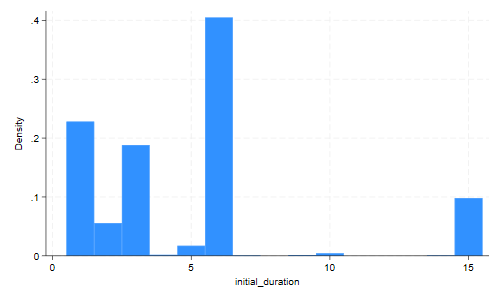
\includegraphics[width=\textwidth]{graphs/it_pat_1902_dur_init.png}
%        \caption{Caption for figure 1}
        \label{fig:figure1}
    \end{minipage}\hfill
    \begin{minipage}{0.32\textwidth}
        \centering
        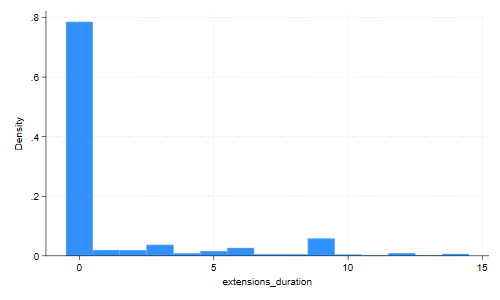
\includegraphics[width=\textwidth]{graphs/it_pat_1902_dur_ext.png}
%        \caption{Caption for figure 2}
        \label{fig:figure2}
    \end{minipage}\hfill
    \begin{minipage}{0.32\textwidth}
        \centering
        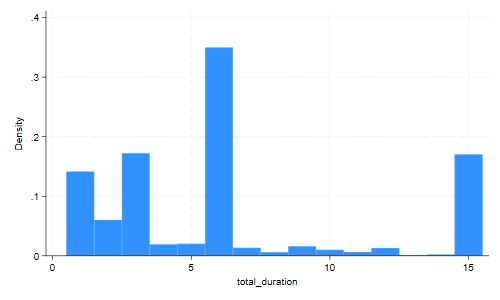
\includegraphics[width=\textwidth]{graphs/it_pat_1902_dur_tot.png}
 %       \caption{Caption for figure 3}
        \label{fig:figure3}
    \end{minipage}
    \caption{Duration of initial applications (l), extensions (c), and total (r) of Italian patents in 1902. Source: own elaboration on data from Nuvolari and Vasta (2015).}


\end{figure}

\hyperlink{patent_fees}{\beamergotobutton{Return}}
    
\end{frame}

%\begin{frame}
%    \centering
%    \huge
%    Regression Discontinuity Results
%\end{frame}

\begin{frame}
    \frametitle{Results: Exhibitions RD, 1855 (Placebo)}

    \centering
    \begin{minipage}{.75\textwidth}
        \begin{table}[!h]

\caption{\label{tab:rd_analysis_placebo}Placebo Test of Italian Unification on Innovative Activity}
\centering
\resizebox{\linewidth}{!}{
\begin{threeparttable}
\begin{tabular}[t]{lllll}
\toprule
\multicolumn{1}{c}{ } & \multicolumn{2}{c}{Log Innovations} & \multicolumn{2}{c}{Ihs Innovations} \\
\cmidrule(l{3pt}r{3pt}){2-3} \cmidrule(l{3pt}r{3pt}){4-5}
\multicolumn{1}{c}{ } & \multicolumn{1}{c}{No FE} & \multicolumn{1}{c}{FE} & \multicolumn{1}{c}{No FE} & \multicolumn{1}{c}{FE} \\
\cmidrule(l{3pt}r{3pt}){2-2} \cmidrule(l{3pt}r{3pt}){3-3} \cmidrule(l{3pt}r{3pt}){4-4} \cmidrule(l{3pt}r{3pt}){5-5}
  & (1) & (2) & (3) & (4)\\
\midrule
Estimate & -0.025* & -0.020 & -0.035* & -0.023\\
SE (BC) & (0.012) & (0.013) & (0.017) & (0.015)\\
Mean DV Treated 50km & 0.015 & 0.015 & 0.018 & 0.018\\
Mean DV Control 50km & 0.007 & 0.007 & 0.009 & 0.009\\
N (Treated) & 667 & 667 & 667 & 667\\
N (Control) & 1549 & 1549 & 1549 & 1549\\
Bandwidth & 23619.409 & 18088.229 & 24106.902 & 18507.961\\
\bottomrule
\end{tabular}
\begin{tablenotes}[para]
\item \textit{Note: } 
\item Table showing coefficient estimates and bias-corrected standard errors of a placebo test, studying the impact of Italian Unification on innovative activity before unification took place. The dependent variable is log or ihs no. of innovations and the independent (running) variable is distance to the border. The bandwidth is estimated using the MSE-optimal bandwidth from \cite{cattaneo2019practical}. The estimates control for area, angle to border and innovation. Models (2) and (4) are conditional on province fixed effects. *: p < 0.10, **: p < 0.05, ***: p < 0.01.
\end{tablenotes}
\end{threeparttable}}
\end{table}

    \end{minipage}
    
\end{frame}

\begin{frame}
    \frametitle{Results: Exhibitions RD, 1867}

    \centering
    \begin{minipage}{.75\textwidth}
        \begin{table}[!h]

\caption{\label{tab:rd_analysis_number}Estimates of Italian Unification on Innovative Activity}
\centering
\resizebox{\linewidth}{!}{
\begin{threeparttable}
\begin{tabular}[t]{lllll}
\toprule
\multicolumn{1}{c}{ } & \multicolumn{2}{c}{Log Innovations} & \multicolumn{2}{c}{Ihs Innovations} \\
\cmidrule(l{3pt}r{3pt}){2-3} \cmidrule(l{3pt}r{3pt}){4-5}
\multicolumn{1}{c}{ } & \multicolumn{1}{c}{No FE} & \multicolumn{1}{c}{FE} & \multicolumn{1}{c}{No FE} & \multicolumn{1}{c}{FE} \\
\cmidrule(l{3pt}r{3pt}){2-2} \cmidrule(l{3pt}r{3pt}){3-3} \cmidrule(l{3pt}r{3pt}){4-4} \cmidrule(l{3pt}r{3pt}){5-5}
  & (1) & (2) & (3) & (4)\\
\midrule
Estimate & 0.140** & 0.149** & 0.175** & 0.189**\\
SE (BC) & (0.063) & (0.052) & (0.079) & (0.065)\\
Mean DV Treated 50km & 0.083 & 0.083 & 0.103 & 0.103\\
Mean DV Control 50km & 0.062 & 0.062 & 0.078 & 0.078\\
N (Treated) & 667 & 667 & 667 & 667\\
N (Control) & 1549 & 1549 & 1549 & 1549\\
Bandwidth & 41406.168 & 45338.659 & 42289.180 & 46458.038\\
\bottomrule
\end{tabular}
\begin{tablenotes}[para]
\item \textit{Note: } 
\item Table showing coefficient estimates and bias-corrected standard errors of the impact of Italian Unification on innovative activity. The dependent variable is log or ihs no. of innovations and the independent (running) variable is distance to the border. The bandwidth is estimated using the MSE-optimal bandwidth from \cite{cattaneo2019practical}. The estimates control for area, angle to border and innovation. Models (2) and (4) are conditional on province fixed effects. *: p < 0.10, **: p < 0.05, ***: p < 0.01.
\end{tablenotes}
\end{threeparttable}}
\end{table}

%        \begin{table}[!h]

\caption{\label{tab:did_analysis_number}Difference-in-difference Estimates of Unification on Innovation}
\centering
\fontsize{9}{11}\selectfont
\begin{threeparttable}
\begin{tabular}[t]{lcccc}
\toprule
\multicolumn{1}{c}{ } & \multicolumn{2}{c}{OLS} & \multicolumn{2}{c}{Poisson} \\
\cmidrule(l{3pt}r{3pt}){2-3} \cmidrule(l{3pt}r{3pt}){4-5}
  & (1) & (2) & (3) & (4)\\
\midrule
Year (1867) & \num{0.037}*** & \num{0.037}*** & \num{1.345}*** & \num{1.345}***\\
 & (\num{0.006}) & (\num{0.006}) & (\num{0.225}) & (\num{0.226})\\
Veneto & \num{-0.029} & \num{0.063} & \num{-1.248} & \num{1.111}\\
 & (\num{0.021}) & (\num{0.039}) & (\num{0.873}) & (\num{0.741})\\
Year (1867) x Veneto & \num{0.007} & \num{0.007} & \num{-0.130} & \num{-0.130}\\
 & (\num{0.013}) & (\num{0.013}) & (\num{0.367}) & (\num{0.368})\\
Elevation & \num{0.000}*** & \num{0.000}*** & \num{-0.003}*** & \num{-0.004}***\\
 & (\num{0.000}) & (\num{0.000}) & (\num{0.001}) & (\num{0.001})\\
Longitude & \num{-0.021}* & \num{-0.049}** & \num{0.111} & \num{-0.735}\\
 & (\num{0.011}) & (\num{0.022}) & (\num{0.219}) & (\num{0.622})\\
Latitude & \num{0.081}*** & \num{0.083}** & \num{2.126}*** & \num{2.756}***\\
 & (\num{0.026}) & (\num{0.036}) & (\num{0.713}) & (\num{0.979})\\
Area & \num{0.004}*** & \num{0.004}*** & \num{0.021}*** & \num{0.040}***\\
 & (\num{0.001}) & (\num{0.001}) & (\num{0.003}) & (\num{0.005})\\
Angle to Border & \num{0.000} & \num{0.000} & \num{-0.005}* & \num{-0.003}\\
 & (\num{0.000}) & (\num{0.000}) & (\num{0.002}) & (\num{0.002})\\
\midrule
N & \num{4432} & \num{4432} & \num{4432} & \num{4432}\\
Province FE & No & Yes & No & Yes\\
\bottomrule
\multicolumn{5}{l}{\rule{0pt}{1em}* p $<$ 0.1, ** p $<$ 0.05, *** p $<$ 0.01}\\
\end{tabular}
\begin{tablenotes}[para]
\item \textit{Note: } 
\item Dependent variables: Number of innovations in municipality $i$. The coefficient of interest is the Year x Group{Veneto} variable. The control variables are latitude, longitude, elevation, and the analysis is conditional on provinde fixed-effects. Standard errors are clustered at the municipality level.
\end{tablenotes}
\end{threeparttable}
\end{table}

    \end{minipage}
    
\end{frame}

\begin{frame}
    \frametitle{Results: Exhibitions RD, 1867}

    \centering
    \begin{minipage}{.75\textwidth}
        \begin{table}[!h]

\caption{\label{tab:rd_analysis_rank}Estimates of Italian Unification on Innovative Activity}
\centering
\resizebox{\linewidth}{!}{
\begin{threeparttable}
\begin{tabular}[t]{lll}
\toprule
\multicolumn{1}{c}{ } & \multicolumn{1}{c}{No FE} & \multicolumn{1}{c}{FE} \\
\cmidrule(l{3pt}r{3pt}){2-2} \cmidrule(l{3pt}r{3pt}){3-3}
  & (1) & (2)\\
\midrule
Estimate & 496.694*** & 510.245***\\
SE (BC) & (144.114) & (112.830)\\
Mean DV Treated 50km & 227.098 & 227.098\\
Mean DV Control 50km & 254.967 & 254.967\\
N (Treated) & 667 & 667\\
N (Control) & 1549 & 1549\\
Bandwidth & 33300.049 & 36859.734\\
\bottomrule
\end{tabular}
\begin{tablenotes}[para]
\item \textit{Note: } 
\item Table showing coefficient estimates and bias-corrected standard errors of the impact of Italian Unification on innovative activity. The dependent variable is Ranking(no. of innovations) and the independent (running) variable is distance to the border. The bandwidth is estimated using the MSE-optimal bandwidth from \cite{cattaneo2019practical}. The estimates control for area, angle to border and innovation. Models (2) and (4) are conditional on province fixed effects. *: p < 0.10, **: p < 0.05, ***: p < 0.01.
\end{tablenotes}
\end{threeparttable}}
\end{table}

%        \begin{table}[!h]

\caption{\label{tab:did_analysis_rank}Difference-in-difference Estimates of Unification on Innovation (Ranking)}
\centering
\fontsize{9}{11}\selectfont
\begin{threeparttable}
\begin{tabular}[t]{lcccc}
\toprule
\multicolumn{1}{c}{ } & \multicolumn{2}{c}{OLS} & \multicolumn{2}{c}{Poisson} \\
\cmidrule(l{3pt}r{3pt}){2-3} \cmidrule(l{3pt}r{3pt}){4-5}
  & (1) & (2) & (3) & (4)\\
\midrule
Year (1867) & \num{131.938}*** & \num{131.938}*** & \num{1.352}*** & \num{1.352}***\\
 & (\num{21.298}) & (\num{21.342}) & (\num{0.237}) & (\num{0.237})\\
Veneto & \num{-111.120}** & \num{176.963}** & \num{-1.302}** & \num{1.049}*\\
 & (\num{49.439}) & (\num{85.169}) & (\num{0.590}) & (\num{0.589})\\
Year (1867) x Veneto & \num{-39.857} & \num{-39.857} & \num{-0.349} & \num{-0.349}\\
 & (\num{34.806}) & (\num{34.877}) & (\num{0.393}) & (\num{0.394})\\
Elevation & \num{-0.283}*** & \num{-0.332}*** & \num{-0.002}*** & \num{-0.003}***\\
 & (\num{0.052}) & (\num{0.058}) & (\num{0.000}) & (\num{0.001})\\
Longitude & \num{-5.918} & \num{-33.508} & \num{0.251} & \num{0.154}\\
 & (\num{21.974}) & (\num{49.318}) & (\num{0.164}) & (\num{0.469})\\
Latitude & \num{171.749}*** & \num{245.251}*** & \num{1.563}*** & \num{2.552}***\\
 & (\num{51.876}) & (\num{85.851}) & (\num{0.518}) & (\num{0.824})\\
Area & \num{6.111}*** & \num{6.599}*** & \num{0.017}*** & \num{0.027}***\\
 & (\num{1.192}) & (\num{1.254}) & (\num{0.002}) & (\num{0.004})\\
Angle to Border & \num{-0.200} & \num{-0.225} & \num{-0.004}** & \num{-0.003}*\\
 & (\num{0.127}) & (\num{0.141}) & (\num{0.002}) & (\num{0.002})\\
\midrule
N & \num{4432} & \num{4432} & \num{4432} & \num{4432}\\
Province FE & No & Yes & No & Yes\\
\bottomrule
\multicolumn{5}{l}{\rule{0pt}{1em}* p $<$ 0.1, ** p $<$ 0.05, *** p $<$ 0.01}\\
\end{tabular}
\begin{tablenotes}[para]
\item \textit{Note: } 
\item Dependent variables: Rank(number of innovations) in municipality $i$, where higher is more innovative. The coefficient of interest is the Year x Group{Veneto} variable. The control variables are latitude, longitude, elevation, and the analysis is conditional on provinde fixed-effects. Standard errors are clustered at the municipality level.
\end{tablenotes}
\end{threeparttable}
\end{table}

    \end{minipage}
    
\end{frame}

\begin{frame}
    \frametitle{Results: Exhibitions RD, 1867}

    \centering
    \begin{minipage}{.75\textwidth}
        \begin{table}[!h]

\caption{\label{tab:rd_analysis_dummy}Estimates of Italian Unification on Innovative Activity}
\centering
\resizebox{\linewidth}{!}{
\begin{threeparttable}
\begin{tabular}[t]{lll}
\toprule
\multicolumn{1}{c}{ } & \multicolumn{1}{c}{No FE} & \multicolumn{1}{c}{FE} \\
\cmidrule(l{3pt}r{3pt}){2-2} \cmidrule(l{3pt}r{3pt}){3-3}
  & (1) & (2)\\
\midrule
Estimate & 0.114*** & 0.117***\\
SE (BC) & (0.033) & (0.026)\\
Mean DV Treated 50km & 0.052 & 0.052\\
Mean DV Control 50km & 0.058 & 0.058\\
N (Treated) & 667 & 667\\
N (Control) & 1549 & 1549\\
Bandwidth & 33151.481 & 36876.632\\
\bottomrule
\end{tabular}
\begin{tablenotes}[para]
\item \textit{Note: } 
\item Table showing coefficient estimates and bias-corrected standard errors of the impact of Italian Unification on innovative activity. The dependent variable is Dummy(no. of innovations > 0) and the independent (running) variable is distance to the border. The bandwidth is estimated using the MSE-optimal bandwidth from \cite{cattaneo2019practical}. The estimates control for area, angle to border and innovation. Models (2) and (4) are conditional on province fixed effects. *: p < 0.10, **: p < 0.05, ***: p < 0.01.
\end{tablenotes}
\end{threeparttable}}
\end{table}

%        \begin{table}[!h]

\caption{\label{tab:did_analysis_dummy}Difference-in-difference Estimates of Unification on Indicator Innovation}
\centering
\fontsize{9}{11}\selectfont
\begin{threeparttable}
\begin{tabular}[t]{lcccc}
\toprule
\multicolumn{1}{c}{ } & \multicolumn{2}{c}{OLS} & \multicolumn{2}{c}{Poisson} \\
\cmidrule(l{3pt}r{3pt}){2-3} \cmidrule(l{3pt}r{3pt}){4-5}
  & (1) & (2) & (3) & (4)\\
\midrule
Year (1867) & \num{0.030}*** & \num{0.030}*** & \num{1.371}*** & \num{1.371}***\\
 & (\num{0.005}) & (\num{0.005}) & (\num{0.242}) & (\num{0.243})\\
Veneto & \num{-0.026}** & \num{0.040}** & \num{-1.320}** & \num{1.053}*\\
 & (\num{0.011}) & (\num{0.019}) & (\num{0.599}) & (\num{0.595})\\
Year (1867) x Veneto & \num{-0.009} & \num{-0.009} & \num{-0.359} & \num{-0.359}\\
 & (\num{0.008}) & (\num{0.008}) & (\num{0.401}) & (\num{0.402})\\
Elevation & \num{0.000}*** & \num{0.000}*** & \num{-0.002}*** & \num{-0.003}***\\
 & (\num{0.000}) & (\num{0.000}) & (\num{0.000}) & (\num{0.001})\\
Longitude & \num{-0.001} & \num{-0.007} & \num{0.257} & \num{0.168}\\
 & (\num{0.005}) & (\num{0.011}) & (\num{0.165}) & (\num{0.473})\\
Latitude & \num{0.039}*** & \num{0.056}*** & \num{1.577}*** & \num{2.582}***\\
 & (\num{0.012}) & (\num{0.020}) & (\num{0.524}) & (\num{0.834})\\
Area & \num{0.001}*** & \num{0.001}*** & \num{0.017}*** & \num{0.027}***\\
 & (\num{0.000}) & (\num{0.000}) & (\num{0.002}) & (\num{0.004})\\
Angle to Border & \num{0.000} & \num{0.000} & \num{-0.004}** & \num{-0.003}*\\
 & (\num{0.000}) & (\num{0.000}) & (\num{0.002}) & (\num{0.002})\\
\midrule
N & \num{4432} & \num{4432} & \num{4432} & \num{4432}\\
Province FE & No & Yes & No & Yes\\
\bottomrule
\multicolumn{5}{l}{\rule{0pt}{1em}* p $<$ 0.1, ** p $<$ 0.05, *** p $<$ 0.01}\\
\end{tabular}
\begin{tablenotes}[para]
\item \textit{Note: } 
\item Dependent variables: Dummy(Number of innovations > 1) in municipality $i$. The coefficient of interest is the Year x Group{Veneto} variable. The control variables are latitude, longitude, elevation, and the analysis is conditional on provinde fixed-effects. Standard errors are clustered at the municipality level.
\end{tablenotes}
\end{threeparttable}
\end{table}

    \end{minipage}
    
\end{frame}

\begin{frame}
\begin{table}[!h]
\caption{The Lombardo-Venetian provinces, 1857-1823 (TO BE UPDATED)}
\centering
\fontsize{8}{8}\selectfont

    \begin{tabular}{l r r r r r r}  
        \toprule
        Province & Pop. & Pop./Ha & Urb. & Agr. & Ind. & Serv.    \\ 
        \midrule
        Bergamo & 0.39 & 0.98 & 0.07 & 0.68 & 0.17 & 0.15 \\
        \textit{Brescia} & 0.36 & 1.16 & 0.12 & 0.54 & 0.23 & 0.23 \\
        Como & 0.44 & 1.60 & 0.04 & 0.71 & 0.16 & 0.13 \\
        Cremona & 0.21 & 1.57 & 0.14 & 0.59 & 0.22 & 0.19 \\
        Lodi e Crema & 0.22 & 1.90 & 0.08 & 0.6 & 0.21 & 0.2 \\
        \textit{Mantova} & 0.26 & 1.13 & 0.11 & 0.65 & 0.19 & 0.16 \\
        Milano & 0.48 & 2.59 & 0.29 & 0.64 & 0.18 & 0.19 \\
        Pavia & 0.18 & 1.80 & 0.16 & 0.60 & 0.21 & 0.19 \\
        Sondrio & 0.10 & 0.32 & .00 & 0.76 & 0.13 & 0.11 \\
        \textbf{Lombardy} & 2.66 & 1.45 & 0.11 & 0.64 & 0.19 & 0.17 \\
         &  & &  &  &  \\
        Belluno & 0.15 & 0.48 & 0.07 & 0.72 & 0.18 & 0.10 \\
        Padova & 0.31 &1.45 & 0.18 & 0.57 & 0.29 & 0.15 \\
        Rovigo & 0.17 & 1.58 & 0.07 & 0.65 & 0.23 & 0.13 \\
        Treviso & 0.30 & 1.23 & 0.07 & 0.71 & 0.16 & 0.13 \\
        Udine & 0.43 & 0.65 & 0.05 & 0.70 & 0.19 & 0.11 \\
        Venezia & 0.30 & 1.18 & 0.47 & 0.38 & 0.4 & 0.22 \\
        \textit{Verona} & 0.31 & 1.11 & 0.17 & 0.53 & 0.31 & 0.16 \\
        Vicenza & 0.32 & 1.12 & 0.17 & 0.58 & 0.27 & 0.15 \\
        \textbf{Veneto} & 2.29 & 1.10 & 0.16 & 0.61 & 0.25 & 0.14 \\
        \bottomrule    
    \end{tabular}
    
    Source: own calculations and Chilosi and Ciccarelli (2021), based on Castiglioni (1862). Note: Urb. is the share of pop. living in towns of 10K or more.
    Note: 1821 census for Lombardy, 1823 for Veneto. 

\end{table}
 
\end{frame}

\end{document}

